\section{Missbrauch des „Wo ist?“ Dienstes}
\label{sec:Missbrauch}

Das Hauptangriffsziel für Angreifer des „Wo ist?“ Dienstes sind die Standortdaten der Nutzer.
Apple ergreift verschiedene Maßnahmen, um die Sicherheit der Standortdaten sicherzustellen, wie bei der Erläuterung der Funktionsweise in \autoref{sec:Funktionsweise_FindMy} bereits gezeigt wurde.
Untersuchungen, wie durch Tonetto \textit{et al.} \cite{Tonetto_FindMy} haben jedoch gezeigt, dass dennoch Missbrauchspotenzial besteht, gegen welches der Dienst nicht oder nicht ausreichend geschützt ist.
\autoref{tab:cia_findmy} zeigt die allgemeinen \textit{CIA}-Sicherheitsziele Vertraulichkeit (\textit{\textbf{C}onfidentiality}), Integrität (\textit{\textbf{I}ntegrity}) und Verfügbarkeit (\textit{\textbf{A}vailability}) sowie mögliche Angriffsziele im Kontext des „Wo ist?“ Dienstes.
Untersuchungen von Angriffen und Missbrauchsszenarien im Folgenden verweisen jeweils auf die betroffenen Sicherheitsziele.

\begin{table}[ht]
  \caption{Sicherheitsziele des „Wo ist?“ Dienstes und mögliche Angriffsziele.}
  \label{tab:cia_findmy}
  \begin{tabularx}{\textwidth}{ |l|X|X| }
    \hline
    \textbf{Sicherheitsziel}  & \textbf{Beschreibung}                                               & \textbf{Angriffsziel}                                           \\
    \Xhline{0.5mm}
    \hline
    Vertraulichkeit           & Standortdaten sind nur befugten Personen zugänglich.                & Standort eines Nutzers oder eines Geräts erhalten.              \\
    \hline
    Integrität                & Standortdaten sind vor Manipulation geschützt.                      & Standortdaten eines Nutzers oder eines Geräts manipulieren.     \\
    \hline
    Verfügbarkeit             & Standortdaten können abgerufen werden.                              & Verhindern, dass Standortdaten abgerufen werden können.         \\
    \hline
  \end{tabularx}
\end{table}
Auf Basis dieser Sicherheitsziele wird gezeigt, wie die von Apple implementierten Sicherheitsmaßnahmen, viele Angriffsszenarien erfolgreich unterbinden können.
Im Anschluss werden in \autoref{sec:szenarien} konkrete Missbrauchsszenarien und mögliche Gegenmaßnahmen erläutert.

Die von Heinrich \textit{et al.} \cite{Heinrich_FindMy} identifizierten Angreifermodelle in \autoref{fig:adversary_models} zeigen verschiedene Wege, wie Angreifer mit unterschiedlichen Möglichkeiten versuchen können, den Dienst anzugreifen.
Sie gehen von vier verschiedenen Angreifermodellen aus, die sich in den Möglichkeiten des Angreifers unterscheiden.
Potenzielle Angriffe können demnach von lokal installierten Anwendungen, Geräten in \ac{BLE}-Reichweite, einem klassischen Netzwerkangreifer und dem Dienstanbieter, also von Apple ausgehen.
Für jedes Angreifermodell werden verschiedene mögliche Ziele definiert.
\begin{figure}[ht]
  \centering
  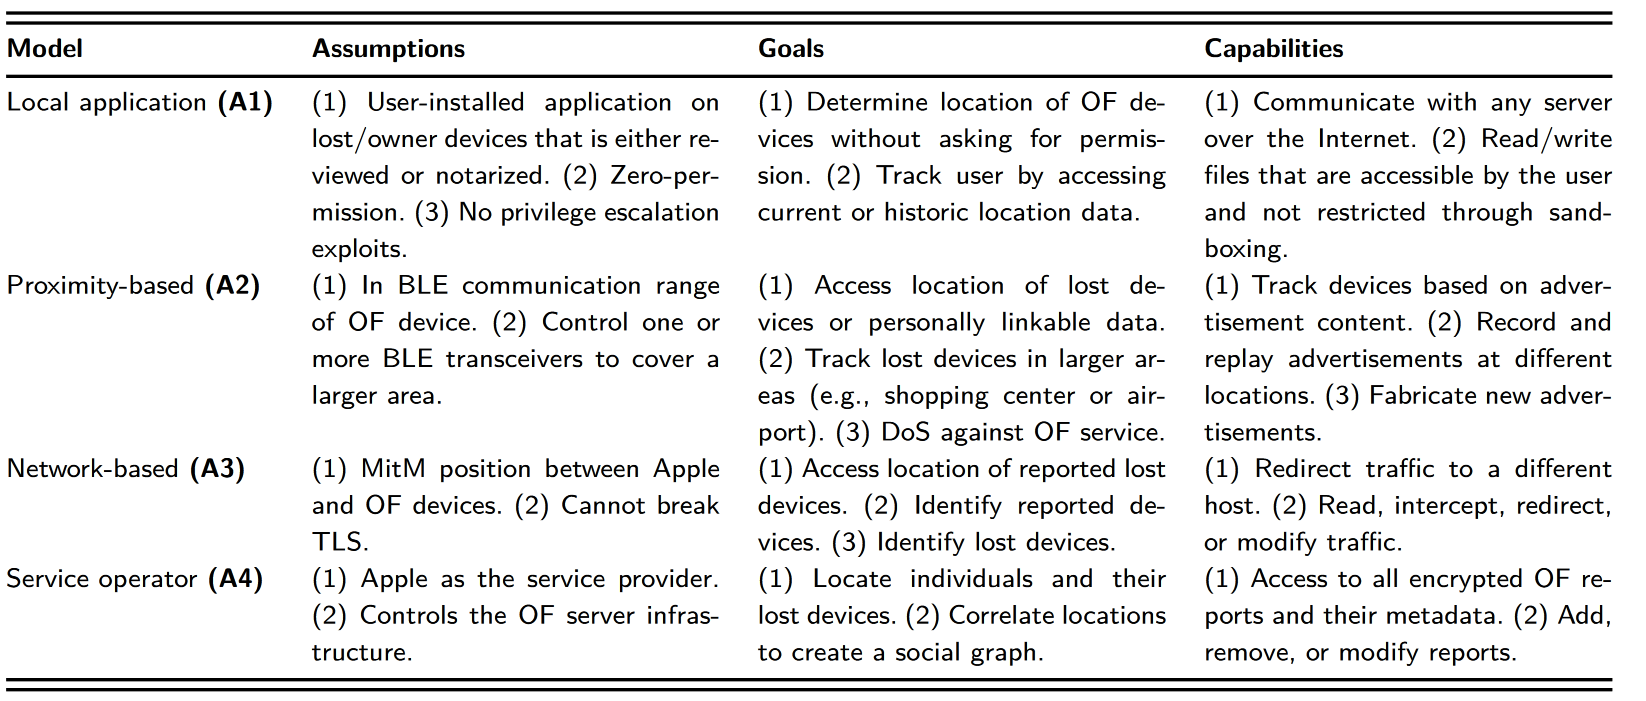
\includegraphics[width=\textwidth]{img/adversary_models}
  \caption{Angreifermodelle für den „Wo ist?“ Dienst \cite{Heinrich_FindMy}.}
  \label{fig:adversary_models}
\end{figure}

\autoref{tab:cia_adversary_models} ordnet den Zielen der einzelnen Angreifermodelle die betroffenen Sicherheitsziele zu.
\begin{table}[h]
  \caption{Zuordnung der Ziele der Angreifermodelle zu den allgemeinen Sicherheitszielen.}
  \label{tab:cia_adversary_models}
  \centering

  \begin{tabularx}{\textwidth}{ |l|X|X|l|X| }
    \hline
    \textbf{Angreifermodell}  & \textbf{Ziel} & \textbf{Vertraulichkeit} & \textbf{Integrität} & \textbf{Verfügbarkeit} \\
    \Xhline{0.5mm}
    \hline
    \multirow{2}{*}{A1} & (1) & \cmark & & \\
    \cline{2-5}
    & (2) & \cmark & & \\
    \hline
    \multirow{3}{*}{A2} & (1) & \cmark & & \\
    \cline{2-5}
    & (2) & \cmark & & \\
    \cline{2-5}
    & (3) & & (\cmark) & \cmark  \\
    \hline
    \multirow{3}{*}{A3} & (1) & \cmark & & \\
    \cline{2-5}
    & (2) & \cmark & & \\
    \cline{2-5}
    & (3) & \cmark & & \\
    \hline
    \multirow{2}{*}{A1} & (1) & \cmark & & \\
    \cline{2-5}
    & (2) & \cmark & & \\
    \hline
  \end{tabularx}
\end{table}
Dabei fällt auf, dass der Fokus auf der Vertraulichkeit der Daten liegt.
Bei der Erläuterung der Sicherheitsmaßnahmen im Folgenden wird deutlich, dass auch bei der Wahl von Maßnahmen durch Apple der Fokus auf der Vertraulichkeit liegt.
Somit ist davon auszugehen, dass beim Design des Dienstes ähnliche Angreifermodelle zugrunde gelegt wurden.
Sollten Angreifer Zugriff auf die Standortdaten erhalten, könnten sie diese für viele verschiedene Zwecke missbrauchen.
Zum Beispiel können diese Daten für gezielte Diskriminierung, Verfolgung und Überwachung durch Dritte oder auch durch staatliche Akteure verwendet werden.
Als personenbezogene Daten unterliegen die Standortdaten zusätzlich der \ac{DSGVO}.
Durch mögliche Rückschlüsse auf beispielsweise religiöse oder politische Überzeugungen sind Standortdaten nach Artikel 9 \ac{DSGVO} häufig auch als sensible personenbezogene Daten zu betrachten.
Deshalb ist Apple zumindest innerhalb der Europäischen Union auch verpflichtet, die Vertraulichkeit der Daten durch geeignete Maßnahmen zu schützen.
Wie bereits in \autoref{sec:Funktionsweise_FindMy} gezeigt, trifft Apple verschiedene Maßnahmen, die darauf abzielen die Vertraulichkeit zu wahren.
Die Auswirkungen dieser Maßnahmen werden in \autoref{sec:auswirkungen_sicherheitsmassnahmen} näher betrachtet.

Angriffe auf die Integrität und die Verfügbarkeit der Daten werden \cite{Heinrich_FindMy} nicht detailliert untersucht.
Nur das \textit{Proximity-based} Modell (A2 in \autoref{tab:cia_adversary_models}) zielt auch auf die Integrität und die Verfügbarkeit der Daten ab.
Wird die Verfügbarkeit beeinträchtigt, ist es für den Besitzer eines Geräts nicht mehr möglich, die aktuellen Standortdaten abzurufen.
Beide Sicherheitsziele sind hier eng miteinander verbunden.
Die Beeinträchtigung der Integrität durch Manipulation von Standortdaten führt beispielsweise dazu, dass der Besitzer nicht zwischen korrekten und manipulierten Daten unterscheiden kann.
Damit sind für den Besitzer keine zuverlässigen Standortdaten verfügbar.
Inwieweit Apples Sicherheitsmaßnahmen auch Integrität und Verfügbarkeit schützen, und welche Angriffe dennoch möglich sind, wird in \autoref{sec:auswirkungen_sicherheitsmassnahmen} und \autoref{sec:szenarien} näher betrachtet.
Außerdem wird in diesem Zusammenhang gezeigt, dass die von Heinrich \textit{et al.} \cite{Heinrich_FindMy} identifizierten Angreifermodelle nicht ausreichen, um alle hier aufgeführten Missbrauchsszenarien zu klassifizieren.

\subsection{Auswirkungen der Sicherheitsmaßnahmen}
\label{sec:auswirkungen_sicherheitsmassnahmen}

\subsubsection{Ende-zu-Ende-Verschlüsselung}
Die Betrachtung der Funktionsweise in \autoref{sec:Funktionsweise_FindMy} zeigt, wie die Ende-zu-Ende-Verschlüsselung des Dienstes technisch umgesetzt wird.
Unter den Annahmen, dass ein Angreifer die Verschlüsselung nicht brechen kann und dass die Synchronisierung der \acp{MBK} über die iCloud-Keychain sicher ist, ist gewährleistet, dass nur der Besitzer des verlorenen Geräts dieses lokalisieren kann.
Auch wenn ein Angreifer direkt auf Apples Server zugreifen könnte oder die Daten auf dem Transportweg abgreifen könnte, sind die Standortinformationen der Lost Devices sicher.
Da die Entschlüsselung nur auf Owner Devices durch die sicher gespeicherten \acp{MBK} möglich ist, sind unverschlüsselte Standortinformationen niemals außerhalb eines Owner Devices verfügbar.
Als weitere Sicherheitsmaßnahme werden \ac{MITM}-Angriffe, bei der Kommunikation mit Apples Servern, durch die Verwendung von \ac{TLS}-verschlüsselten Verbindungen mit Certificate Pinning verhindert \cite{Heinrich_FindMy}.
Durch die Ende-zu-Ende-Verschlüsselung werden somit alle vom Netzwerkangreifer (A3 in \autoref{fig:adversary_models}) ausgehenden Bedrohungen adressiert.
Da lokale unprivilegierte Apps keinen Zugriff auf die in der iCloud-Keychain des Besitzers gespeicherten Schlüssel haben, werden so auch die von  lokalen Angreifern (A1 in \autoref{fig:adversary_models}) ausgehenden Bedrohungen behandelt.
Eine in \cite{Heinrich_FindMy} aufgedeckte Schwachstelle, die aufgrund von unsicherer Speicherung der Schlüssel unbefugten Zugriff auf die entschlüsselten Standortdaten ermöglichte, wurde durch Apple mittlerweile behoben.

Zusätzlich macht es die Ende-zu-Ende-Verschlüsselung auch Apple unmöglich, die Standortdaten der Nutzer zu entschlüsseln, womit das Lokalisieren durch den Dienstanbieter (Ziel (1) von A4 in \autoref{fig:adversary_models}) verhindert wird.
Außerdem verbessert die Verschlüsselung die Integrität der Daten, da einmal verschlüsselte Daten ohne Entschlüsselung nicht manipuliert werden können, ohne dass diese Manipulation erkannt werden kann.


\subsubsection{Schlüsselrotation}
Die Schlüsselrotation der Advertising Keys im Intervall von 15 Minuten bei Endgeräten und im Intervall von 24 Stunden bei Accesories, wie in \autoref{sec:Funktionsweise_FindMy} beschrieben, trägt ebenfalls zur Vertraulichkeit der Standortdaten bei.
Durch die regelmäßige Rotation der Schlüssel wird das Tracking von Geräten anhand der im Advertising gesendeten Daten erschwert.
Diese Maßnahme richtet sich gegen das Tracking durch einen Angreifer in der Nähe (A2 mit Ziel (2) in \autoref{fig:adversary_models}).
Außerdem müssten für einen solchen Angriff viele scannende Geräte so positioniert werden, dass auch bei Bewegung die Advertisement-Pakete des zu verfolgenden Geräts von einem der Scanner erfasst wird.
Um größere Bereiche abzudecken, wären jedoch sehr viele scannende Geräte notwendig, was den Angriff bereits deutlich erschwert.
In Verbindung mit der Schlüsselrotation ist die Verfolgung, auch mit hohem Aufwand, nur für das Intervall der Schlüsselrotation möglich.
Allerdings können AirTags und Drittanbieterprodukte durch das längere Intervall für bis zu 24 Stunden verfolgt werden.
Für Angreifer ist der Angriff jedoch insgesamt sehr aufwändig, sodass eine direkte Verfolgung des Opfers in den meisten Fällen praktikabler wäre.
Heinrich \textit{et al.} \cite{Heinrich_FindMy} betrachten die Schlüsselrotation als ausreichend, um die Verfolgung von Geräten nach diesem Muster zu verhindern.
Jedoch waren zum Zeitpunkt ihrer Analyse keine Geräte mit einem Intervall der Schlüsselrotation von mehr als 15 Minuten auf dem Markt.
Es ist unklar, ob die Autoren auch ein Rotationsintervall von 24 Stunden als ausreichend bewerten würden.